\documentclass[11pt, oneside]{article} 	% use "amsart" instead of "article" for AMSLaTeX format
\usepackage{geometry} 		% See geometry.pdf to learn the layout options. There are lots.
\geometry{letterpaper} 		% ... or a4paper or a5paper or ... 
\usepackage[parfill]{parskip} 		% Activate to begin paragraphs with an empty line rather than an indent
\usepackage{graphicx}				% Use pdf, png, jpg, or eps§ with pdflatex; use eps in DVI mode
								% TeX will automatically convert eps --> pdf in pdflatex		
\usepackage{amssymb}
\usepackage{amsmath}
\usepackage{authblk}
\usepackage{framed}
\usepackage[
backend=biber,
style=alphabetic,
]{biblatex}
\usepackage{graphicx}
\graphicspath{ {./images/} }
\usepackage{verbatim}
\usepackage{tikz} 
\usepackage{xcolor,colortbl}
\usepackage{subcaption}
\captionsetup{compatibility=false}
\usepackage{syntonly}


\title{Spotting Graph Theory Problems in Spot It}
\author[1]{Dave Fetterman}
\author[2]{James Wang}
\affil[1]{Obviously Unemployed}
\affil[2]{Surprisingly Employed}

\date{3/29/23}
\begin{document}
\maketitle

\begin{abstract}

Main plan:
\begin{itemize}
\item Explain the game
\item Modeling with a graph.  Tiling $C_n$ with $C_g$'s.
\item Set up the problem - s and g determine everything, what combos work?
\item The Candidate Theorem: What combos CAN work?
\item Showing combos with 3.
\item Complete graph of setup  g = s - 1.  Introduce: round robin squares.  Show s = 5, g=4
\item Complete graphs of setup g = s.  Show s = 3, g = 3.
\item TODO: Chopping s 
\item Notes on nonuniform g sizes (removal, inception, the actual game of Spot It)
\end{itemize}

\end{abstract}

\section{The Game}

\section{The Graph Theorem}

\begin{framed}
A deck of $n$ Spot It cards with $m$ symbols over $s$ slots can be represented by a graph $G$ on $n$ nodes of degree $s$ and edges of $m$ unique colors, and for any color $m_i$, the edges of that color (and all adjacent nodes) form a complete subgraph of $G_i$ of $G$. 
\end{framed}

Note: Self-loop objection.

\section{The Core Question}

\begin{framed}
For what choices of $g$ and $s$ can graphs be constructed that satisfy our constraints? 
\end{framed}

TODO

\section{The Candidate Theorem}

\begin{framed}
Suppose further that that every symbol $s$ has exactly $g$ cards containing it \footnote{for example, all $s=7$ symbols in the graph above correspond to cliques of size $g=3$}.  Then \begin{enumerate}
\item Total nodes $n = (g-1)s + 1$, 
\item Total colors $m = \frac{{n \choose 2}}{{g \choose 2}}$.
\item $g | s(s-1)$.
\item If $s >1 $ and $g > 1$ then $g \leq s$ 
\item All candidate configurations of $g, s$ are $g \leq s$, $g | s(s-1)$.
\end{enumerate}
\end{framed}

\emph{Proof}:
\begin{enumerate}
\item As in Fig. 1, node $n_0$'s adjacencies are exactly $s$ monocolor cliques of size $g-1$ (excluding $n_0$ itself).  In a complete graph, these adjacencies comprise the total node set, so $n = (g-1)s + 1$ when adding $n_0$ back in.  Using any other node is equivalent.
\item A complete graph $C_n$'s has ${n \choose 2}$ edges.  A monocolor clique of size $g$ is a complete graph as well, with ${g \choose 2}$ edges.  $C_n$'s edges are exactly these equal-sized cliques, so there are therefore $m = \frac{{n \choose 2}}{{g \choose 2}}$ of them.
\item 
\begin{align}
{g \choose 2} | {n \choose 2} \Rightarrow \frac{n(n-1)}{g(g-1)} \in \mathbb{N} \Rightarrow g(g-1) | n(n-1) \\
 n = (g-1)s+1 \Rightarrow g(g-1) | (sg-s+1)(sg-s) = (sg-s+1)s(g-1)\\
\Rightarrow g | s^2g - s^2 + s \Rightarrow g | (1-s)s \Rightarrow g | s(s-1) 
\end{align}
\item Any node $n_i$ is adjacent to $s$ monocolor cliques of size $g$.  These cliques $C_1 ... C_g$, containing non-$n_i$ nodes if $g > 1$, comprise all nodes, and any other cliques can contain no more than one of each $C_i$.  This means that clique of size $g$ greater than $s$ cannot be formed, since the only place to find nodes are these $C_1 ... C_g$.  The other trivial case, $s=1$, means there is only one color in the whole graph. 
\\

This means we need not consider configurations like $g = 6, s=3$ even though $6 | 3(3-1)$.
\\
Another corollary here is that \fbox{$m \geq n$}, since:
\begin{align}
n = (sg - s + 1) \\
m = \frac{{(sg - s + 1)(sg-s) \choose 2}}{{g \choose 2}} = \frac{(sg-s+1)(sg-s)}{g(g-1)} = \frac{(sg-s+1)s}{g} \\
\Rightarrow m = (\frac{s}{g})n\\
s \geq g \Rightarrow m \geq n
\end{align}
\end{enumerate}

For example, a tiling of triangles ($g=3$) means that either $s \equiv 0 \mod 3$ or $s \equiv 1 \mod 3$.  
\\
Since $n = (g-1)s + 1 = 2s + 1$ or $n \equiv 1 \mod 2$, then $n = 2(3k) + 1 = 6k+1$ or $n = 2(3k+1) + 1 = 6k+3$, meaning $n \in \{1,3\} \mod 6$.


\section{Some examples with $g=3$}

\begin{figure}
\centering
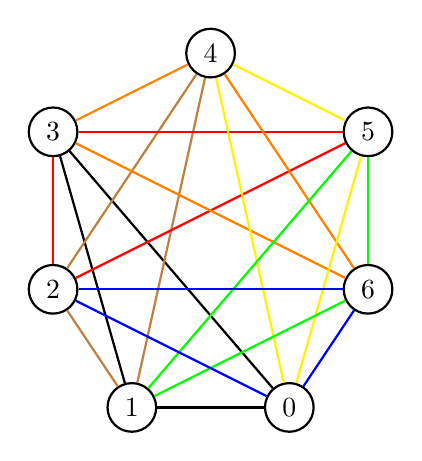
\begin{tikzpicture}
\begin{scope}[every node/.style={circle,thick,draw}]
  \node (0) at (3,0.5) {0};
  \node (1) at (1,0.5) {1};
  \node (2) at (0,2) {2};
  \node (3) at (0,4) {3};
  \node (4) at (2,5) {4};
  \node (5) at (4,4) {5};
  \node (6) at (4,2) {6};
  
  
\draw[thick, black] (0) -- (1); 
\draw[thick, black] (1) -- (3); 
\draw[thick, black] (0) -- (3); 

\draw[thick, brown] (1) -- (2); 
\draw[thick, brown] (2) -- (4); 
\draw[thick, brown] (1) -- (4); 

\draw[thick, red] (2) -- (3); 
\draw[thick, red] (3) -- (5); 
\draw[thick, red] (2) -- (5); 

\draw[thick, orange] (3) -- (4); 
\draw[thick, orange] (4) -- (6); 
\draw[thick, orange] (3) -- (6); 

\draw[thick, yellow] (4) -- (5); 
\draw[thick, yellow] (5) -- (0); 
\draw[thick, yellow] (4) -- (0); 

\draw[thick, green] (5) -- (6); 
\draw[thick, green] (6) -- (1); 
\draw[thick, green] (5) -- (1); 

\draw[thick, blue] (6) -- (0); 
\draw[thick, blue] (0) -- (2); 
\draw[thick, blue] (6) -- (2); 


\end{scope}

\end{tikzpicture}
\label{fig:3377}
\caption{s=3, g=3, n=7, m=7.  Rule: (i, i+1, i+3) for all i.}
\end{figure}


\begin{figure}
\centering
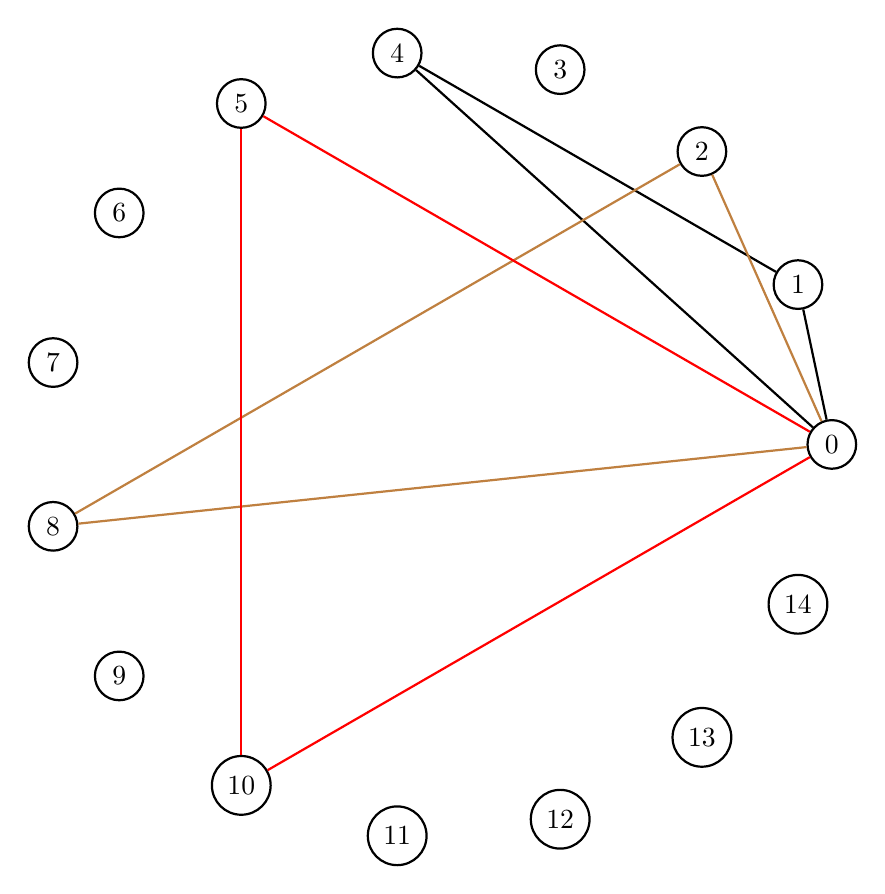
\begin{tikzpicture}
\begin{scope}[every node/.style={circle,thick,draw}]
\node (0) at (5.0, 0.0)  {0}; 
\node (1) at (4.57, 2.03) {1}; 
\node (2) at  (3.35, 3.72) {2}; 
\node (3) at  (1.55, 4.76) {3}; 
\node (4) at  (-0.52, 4.97) {4}; 
\node (5) at  (-2.5, 4.33) {5}; 
\node (6) at  (-4.05, 2.94) {6}; 
\node (7) at  (-4.89, 1.04) {7}; 
\node (8) at  (-4.89, -1.04) {8}; 
\node (9) at  (-4.05, -2.94) {9}; 
\node (10) at  (-2.5, -4.33) {10}; 
\node (11) at  (-0.52, -4.97) {11}; 
\node (12) at  (1.55, -4.76) {12}; 
\node (13) at  (3.35, -3.72) {13}; 
\node (14) at  (4.57, -2.03) {14}; 
  
\draw[thick, black] (0) -- (1); 
\draw[thick, black] (1) -- (4); 
\draw[thick, black] (0) -- (4); 

\draw[thick, brown] (0) -- (2); 
\draw[thick, brown] (2) -- (8); 
\draw[thick, brown] (0) -- (8); 

\draw[thick, red] (0) -- (5); 
\draw[thick, red] (5) -- (10); 
\draw[thick, red] (0) -- (10); 
\end{scope}
,
\end{tikzpicture}
\label{fig:bipartite}
\caption{s=7, g=3, n=15, m=35, node 0 adjacencies.  Rule: (i, i+5, i+10) x 3, (i, i+1, i+4) and (i, i+2, i+8)}
\end{figure}

\begin{itemize}

\item Rule: $g=3, s=3, n=7, m=7: (0,1,3)$
\item Rule: $g=3, s=4, n = 9, m = 12: (0,1,2) \cdot 3; (0,3,6) \cdot 3, (0,5,7) \cdot 3$
\item Rule: Another example: g=3, s=6, n=13, m=26.  3-graphs are at $(i, i+2, i+8)$ and $(i, i+1, i+4)$, addition being $\mod 13$..  NOTE: Is this a subset of s=6, g=6?
\item Rule: $g=3, s=7, n=15, m=35, (i, i+5, i+10) \cdot 3, (i, i+1, i+4), (i, i+2, i+8)$
\item Rule: $g=3, s=9, n=19, m=57: (0,1,6), (0,2,10), (0,3,7)$
\item Rule: $g=3, s=10, n=21, m=70: (0,7,14) \cdot 3, (0,2,10), (0,1,5), (0,3,9)$
\end{itemize}

\section{Generating $g = s-1$, $g \in \mathbb{P}$}
\begin{figure}
\begin{subfigure}{.25\textwidth}
\begin{tabular}{||c c c c||} 
 \hline
$G_0$  & $G_1$ & $G_2$ & $G_3$ \\ [0.5ex] 
 \hline\hline
 0 & 0 & 0 & 0 \\ 
 \hline
 1 & 1 & 1 & 1 \\
 \hline
 2 & 2 & 2  & 2 \\
 \hline
 3 & 3  & 3 & 3 \\
 \hline
\end{tabular}
\caption{$I_0$}
\end{subfigure}
\begin{subfigure}{.25\textwidth}
\begin{tabular}{||c c c c||} 
 \hline
$G_0$  & $G_1$ & $G_2$ & $G_3$ \\ [0.5ex] 
 \hline\hline
 0 & 1 &  2 & 3 \\ 
 \hline
 \cellcolor{green} 1 & \cellcolor{green}  2 &  \cellcolor{green} 3 &  \cellcolor{green} 0 \\
 \hline
 2 & 3 & 0  & 1 \\
 \hline
 3 & 0  & 1 & 2 \\
 \hline
\end{tabular}
\caption{$I_1$}
\end{subfigure}
\begin{subfigure}{.25\textwidth}
\begin{tabular}{||c c c c||} 
 \hline
$G_0$  & $G_1$ & $G_2$ & $G_3$ \\ [0.5ex] 
 \hline\hline
 0 & 2 & 3 & 1 \\ 
 \hline
 1 & 3 & 0 & 2 \\
 \hline
 2 & 0 & 1  & 3 \\
 \hline
 3 & 1  & 2 & 0 \\
 \hline
\end{tabular}
\caption{$I_2$}
\end{subfigure}
\begin{subfigure}{.25\textwidth}
\begin{tabular}{||c c c c||} 
 \hline
$G_0$  & $G_1$ & $G_2$ & $G_3$ \\ [0.5ex] 
 \hline\hline
 0 & 3 & 1 & 2 \\ 
 \hline
 1 & 0 & 2 & 3 \\
 \hline
 2 & 1 & 3  & 0 \\
 \hline
 3 & 2  & 0 & 1 \\
 \hline
\end{tabular}
\caption{$I_3$}
\end{subfigure}
\caption{s=5, g=4 adjacency tables}
\end{figure}


\begin{figure}
\centering
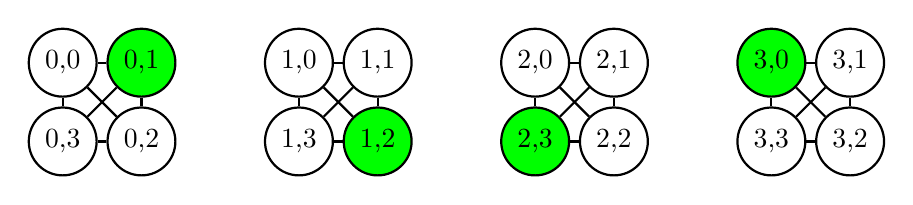
\begin{tikzpicture}
\begin{scope}[every node/.style={circle,thick,draw}]
\node (0) at (0,0)  {0,0}; 
\node (1)[fill=green] at (1,0)  {0,1}; 
\node (2) at (1,-1)  {0,2}; 
\node (3) at (0, -1) {0,3}; 

\draw[thick, black] (0) -- (1); 
\draw[thick, black] (1) -- (2); 
\draw[thick, black] (2) -- (3); 
\draw[thick, black] (3) -- (0); 
\draw[thick, black] (0) -- (2); 
\draw[thick, black] (1) -- (3); 


\node (4) at (3,0)  {1,0}; 
\node (5) at (4,0)  {1,1}; 
\node (6)[fill=green] at (4,-1)  {1,2}; 
\node (7) at (3, -1) {1,3}; 

\draw[thick, black] (4) -- (5); 
\draw[thick, black] (5) -- (6); 
\draw[thick, black] (6) -- (7); 
\draw[thick, black] (7) -- (4); 
\draw[thick, black] (4) -- (6); 
\draw[thick, black] (5) -- (7); 

\node (8) at (6,0)  {2,0}; 
\node (9) at (7,0)  {2,1}; 
\node (10) at (7,-1)  {2,2}; 
\node (11)[fill=green] at (6, -1) {2,3}; 

\draw[thick, black] (8) -- (9); 
\draw[thick, black] (9) -- (10); 
\draw[thick, black] (10) -- (11); 
\draw[thick, black] (11) -- (8); 
\draw[thick, black] (8) -- (10); 
\draw[thick, black] (9) -- (11); 


\node (12)[fill=green] at (9,0)  {3,0}; 
\node (13) at (10,0)  {3,1}; 
\node (14) at (10,-1)  {3,2}; 
\node (15) at (9, -1) {3,3}; 

\draw[thick, black] (12) -- (13); 
\draw[thick, black] (13) -- (14); 
\draw[thick, black] (14) -- (15); 
\draw[thick, black] (15) -- (12); 
\draw[thick, black] (12) -- (14); 
\draw[thick, black] (13) -- (15); 


\end{scope}
\end{tikzpicture}
\caption{TODO: Busted: (TURN THIS TO g=5, s=6) s=5, g=4, n=16, m=20 }
\end{figure}


\begin{figure}
\centering
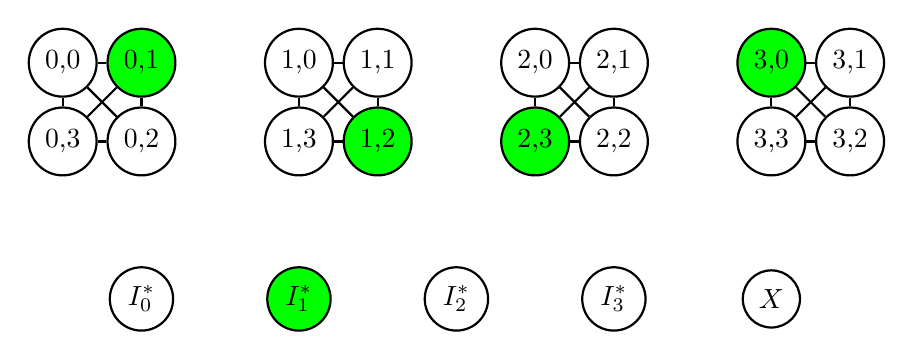
\begin{tikzpicture}
\begin{scope}[every node/.style={circle,thick,draw}]
\node (0) at (0,0)  {0,0}; 
\node (1)[fill=green] at (1,0)  {0,1}; 
\node (2) at (1,-1)  {0,2}; 
\node (3) at (0, -1) {0,3}; 

\draw[thick, black] (0) -- (1); 
\draw[thick, black] (1) -- (2); 
\draw[thick, black] (2) -- (3); 
\draw[thick, black] (3) -- (0); 
\draw[thick, black] (0) -- (2); 
\draw[thick, black] (1) -- (3); 


\node (4) at (3,0)  {1,0}; 
\node (5) at (4,0)  {1,1}; 
\node (6)[fill=green] at (4,-1)  {1,2}; 
\node (7) at (3, -1) {1,3}; 

\draw[thick, black] (4) -- (5); 
\draw[thick, black] (5) -- (6); 
\draw[thick, black] (6) -- (7); 
\draw[thick, black] (7) -- (4); 
\draw[thick, black] (4) -- (6); 
\draw[thick, black] (5) -- (7); 

\node (8) at (6,0)  {2,0}; 
\node (9) at (7,0)  {2,1}; 
\node (10) at (7,-1)  {2,2}; 
\node (11)[fill=green] at (6, -1) {2,3}; 

\draw[thick, black] (8) -- (9); 
\draw[thick, black] (9) -- (10); 
\draw[thick, black] (10) -- (11); 
\draw[thick, black] (11) -- (8); 
\draw[thick, black] (8) -- (10); 
\draw[thick, black] (9) -- (11); 


\node (12)[fill=green] at (9,0)  {3,0}; 
\node (13) at (10,0)  {3,1}; 
\node (14) at (10,-1)  {3,2}; 
\node (15) at (9, -1) {3,3}; 

\draw[thick, black] (12) -- (13); 
\draw[thick, black] (13) -- (14); 
\draw[thick, black] (14) -- (15); 
\draw[thick, black] (15) -- (12); 
\draw[thick, black] (12) -- (14); 
\draw[thick, black] (13) -- (15); 

\node (16) at (1,-3)  {$I_0^*$}; 
\node (17)[fill=green] at (3,-3)  {$I_1^*$}; 
\node (18) at (5,-3)  {$I_2^*$}; 
\node (19) at (7, -3) {$I_3^*$}; 
\node (20) at (9, -3) {$X$}; 

\end{scope}
\end{tikzpicture}
\caption{s=5, g=5}
\end{figure}



\section{Generating $g = s$ for $g-1 \in \mathbb{P}$}

\begin{framed}
TODO: The James construction. 

\end{framed}


TODO Proof



\begin{figure}
\centering
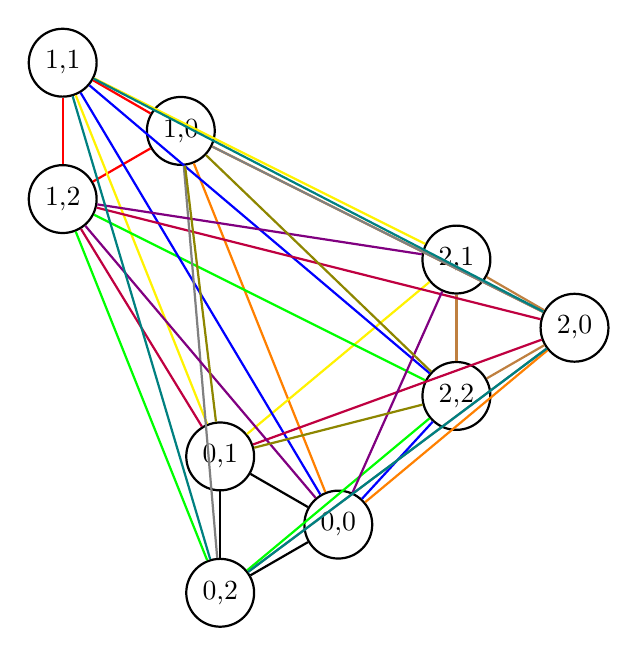
\begin{tikzpicture}
\begin{scope}[every node/.style={circle,thick,draw}]
\node (0) at (1,0)  {0,0}; 
\node (1) at (-.5, .866) {0,1}; 
\node (2) at  (-.5, -.866) {0,2}; 

\draw[thick, black] (0) -- (1); 
\draw[thick, black] (1) -- (2); 
\draw[thick, black] (0) -- (2); 

\node (3) at (-1,5)  {1,0}; 
\node (4) at (-2.5, 5.866) {1,1}; 
\node (5) at  (-2.5, 4.134) {1,2}; 

\draw[thick, red] (3) -- (4); 
\draw[thick, red] (4) -- (5); 
\draw[thick, red] (3) -- (5); 

\node (6) at (4,2.5)  {2,0}; 
\node (7) at (2.5, 3.366) {2,1}; 
\node (8) at  (2.5, 1.634) {2,2}; 

\draw[thick, brown] (6) -- (7); 
\draw[thick, brown] (7) -- (8); 
\draw[thick, brown] (6) -- (8); 


\draw[thick, orange] (0) -- (3); 
\draw[thick, orange] (3) -- (6); 
\draw[thick, orange] (0) -- (6); 


\draw[thick, yellow] (1) -- (4); 
\draw[thick, yellow] (4) -- (7); 
\draw[thick, yellow] (1) -- (7); 


\draw[thick, green] (2) -- (5); 
\draw[thick, green] (5) -- (8); 
\draw[thick, green] (2) -- (8); 



\draw[thick, blue] (0) -- (4); 
\draw[thick, blue] (4) -- (8); 
\draw[thick, blue] (0) -- (8); 


\draw[thick, purple] (1) -- (5); 
\draw[thick, purple] (5) -- (6); 
\draw[thick, purple] (1) -- (6); 


\draw[thick, gray] (2) -- (3); 
\draw[thick, gray] (3) -- (6); 
\draw[thick, gray] (2) -- (6); 


\draw[thick, violet] (0) -- (5); 
\draw[thick, violet] (5) -- (7); 
\draw[thick, violet] (0) -- (7); 


\draw[thick, olive] (1) -- (3); 
\draw[thick, olive] (3) -- (8); 
\draw[thick, olive] (1) -- (8); 


\draw[thick, teal] (2) -- (4); 
\draw[thick, teal] (4) -- (6); 
\draw[thick, teal] (2) -- (6); 


\end{scope}

\end{tikzpicture}
\label{fig:bipartite}
\caption{whole $C_9$: $s=4, g=3, n=9, m=12$}

\end{figure}

\section{A nonexistence result: g=4, s=5}

If we have g=4 and s=5, then there exists a clique of size 4.  Every node of that clique is adjacent to four additional colors, and none of those colors can be shared (else double color edge).
Thus, of the 20 colors, each color has 3 "non-adjacent neighbors".

This forms a graph of n nodes, where each node is a color, and nodes are adjacent if colors share a node in the original graph.  Each node in this graph has degree 3.

Brooks's Theorem\cite{1} states that if every node has degree $\Delta$ or less, than since this is not a complete graph and not an odd cycle, the nodes can be vertex-colored with $\Delta$ or fewer colors, or in this case, 3.  This means that there must NOT be a complete subgraph $K_4$, or four mutually non-adjacent colors.  NOTE: This does not apply as with prime, we end up with connected components of size $K_g$.

Each color offers up exactly 3 non-adjacencies, so we have $20 * 3 / 2 = 30$ non-adjacency edges in the grapjh.
 
Our ``ring'' construction  on which the $(g, s)$ configurations $(p, p+1)$ and $(p+1, p+1)$, $p \in \mathbb{P}$ does not work always if $g \not \mathbb{P}$.

Though we have yet to prove nonexistence for all composite g, we can show that $g=4, s=5$ cannot work.  This is through the proof:
\begin{enumerate}
\item The graph defined by $g=4, s=5 (n=16, m=20)$ must contain four $C_4$ monocolor cliques $S_0, S_1, S_2, S_3$ with no pairwise no overlapping nodes.
\item Any coloring of the graph requires choosing four cliques  $S_0, S_1, S_2, S_3$ plus sixteen cliques $S_i = \{s_{0, i}, s_{1,j}, s_{2, k}, s_{3,l}\}$, with $s_{0, i}$ signifying some node in $S_0$.
\item Such a graph does not exist.
\end{enumerate}

\emph{Proof}: 
\begin{enumerate}
\item 1. Consider that the cliques corresponding to each of the $m=20$ colors must have pairwise overlap of zero or one of the 16 nodes (if they share two nodes, they share an edge, and thus an edge has two colors).  Let's create another graph $G$ where each node $n_i$ corresponds to a color $C_i, i \in [0,19]$ , and an edge $(n_i, n_j)$ exists iff $\{n_i, n_j\} \subseteq C_i, C_j$.  Suppose $G$ has a maximum of three pairwise nonoverlapping cliques.  Then, there can be at most 15 colors, TODO: Did I get this wrong too?
\item TODO
\end{enumerate}

\section{Constructions with mixed g}
\subsection{Trivial}
TODO
\subsection{Chopping}
TODO
\subsection{Inception}
- what about solutions with mixed sized subgraphs? 
You can take the s=7, g=3, n=15, m=35 and change the n, n+5, n+10 triangles into unique colors for s=8, m=45, n=15 and g in {2,3} for example.  


\section{The main question: Are all candidates viable?}

Note: Can drop from$s=4, g=4, n=13, m=13$ to $s=4, g=3, n=9, m=12$ by dropping last $g-$sized clique and all adjacent edges.

\begin{itemize}
\item Perfect difference sets: \url{https://oeis.org/search?q=0+1+3+9+27+49+56+61+77+81&sort=&language=english&go=Search}, \url{https://mathworld.wolfram.com/PerfectDifferenceSet.html}.
\item Necessary for $n = k^2+k+1$.  Sufficient is k being a prime power.
\item We have the rotator of size $g$ iff $g | s-1$, since $gk = s - 1 \Rightarrow s = gk+1 \Rightarrow m = \frac{gk+1}{s}(sg-s+1).$  This means ( I think ) that there are $k(sg-s+1)$ cliques, or $k$ rooted at each node, plus $\frac{sg-s+1}{g}$ other rotator cliques, being $s - \frac{s-1}g$ of size $g$ that are like the island triangles

\end{itemize}



\section{Further questions}

% ======= BONEYARD =======
% ======= BONEYARD =======
% ======= BONEYARD =======
% ======= BONEYARD =======
% ======= BONEYARD =======
% ======= BONEYARD =======
% DF NOTE: These are leftovers from the Dino Paper work, easy to pick up and use if needed.

\begin{comment}


\begin{figure}
\centering
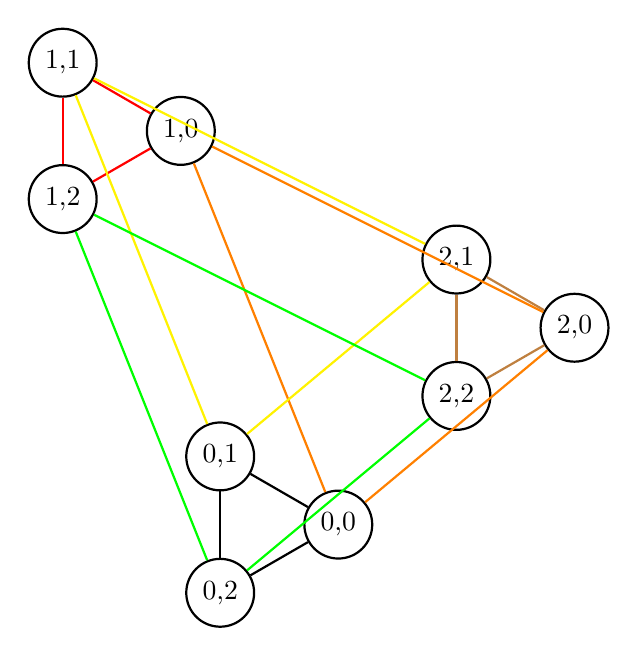
\begin{tikzpicture}
\begin{scope}[every node/.style={circle,thick,draw}]
\node (0) at (1,0)  {0,0}; 
\node (1) at (-.5, .866) {0,1}; 
\node (2) at  (-.5, -.866) {0,2}; 

\draw[thick, black] (0) -- (1); 
\draw[thick, black] (1) -- (2); 
\draw[thick, black] (0) -- (2); 

\node (3) at (-1,5)  {1,0}; 
\node (4) at (-2.5, 5.866) {1,1}; 
\node (5) at  (-2.5, 4.134) {1,2}; 

\draw[thick, red] (3) -- (4); 
\draw[thick, red] (4) -- (5); 
\draw[thick, red] (3) -- (5); 

\node (6) at (4,2.5)  {2,0}; 
\node (7) at (2.5, 3.366) {2,1}; 
\node (8) at  (2.5, 1.634) {2,2}; 

\draw[thick, brown] (6) -- (7); 
\draw[thick, brown] (7) -- (8); 
\draw[thick, brown] (6) -- (8); 

\draw[thick, orange] (0) -- (3); 
\draw[thick, orange] (3) -- (6); 
\draw[thick, orange] (0) -- (6); 


\draw[thick, yellow] (1) -- (4); 
\draw[thick, yellow] (4) -- (7); 
\draw[thick, yellow] (1) -- (7); 


\draw[thick, green] (2) -- (5); 
\draw[thick, green] (5) -- (8); 
\draw[thick, green] (2) -- (8); 





\end{scope}

\end{tikzpicture}
\label{fig:bipartite}
\caption{complete graphs with increment 0}
\end{figure}


\begin{figure}
\centering
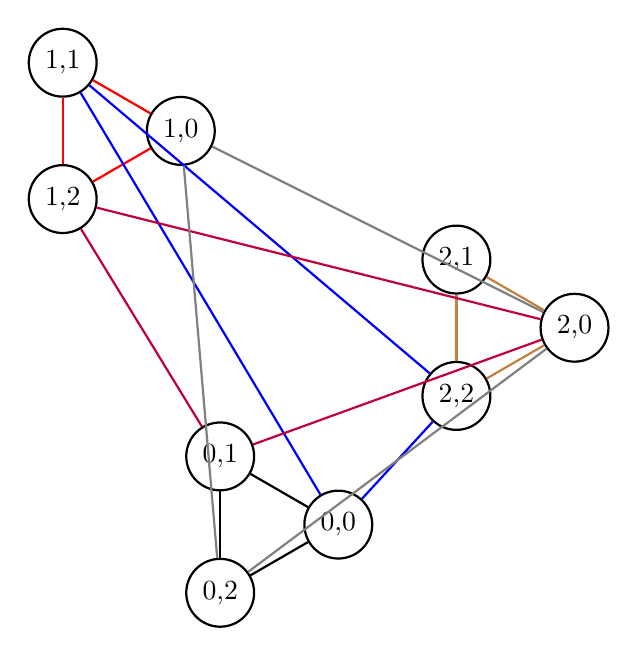
\begin{tikzpicture}
\begin{scope}[every node/.style={circle,thick,draw}]
\node (0) at (1,0)  {0,0}; 
\node (1) at (-.5, .866) {0,1}; 
\node (2) at  (-.5, -.866) {0,2}; 

\draw[thick, black] (0) -- (1); 
\draw[thick, black] (1) -- (2); 
\draw[thick, black] (0) -- (2); 

\node (3) at (-1,5)  {1,0}; 
\node (4) at (-2.5, 5.866) {1,1}; 
\node (5) at  (-2.5, 4.134) {1,2}; 

\draw[thick, red] (3) -- (4); 
\draw[thick, red] (4) -- (5); 
\draw[thick, red] (3) -- (5); 

\node (6) at (4,2.5)  {2,0}; 
\node (7) at (2.5, 3.366) {2,1}; 
\node (8) at  (2.5, 1.634) {2,2}; 

\draw[thick, brown] (6) -- (7); 
\draw[thick, brown] (7) -- (8); 
\draw[thick, brown] (6) -- (8); 

\draw[thick, blue] (0) -- (4); 
\draw[thick, blue] (4) -- (8); 
\draw[thick, blue] (0) -- (8); 


\draw[thick, purple] (1) -- (5); 
\draw[thick, purple] (5) -- (6); 
\draw[thick, purple] (1) -- (6); 


\draw[thick, gray] (2) -- (3); 
\draw[thick, gray] (3) -- (6); 
\draw[thick, gray] (2) -- (6); 
\end{scope}

\end{tikzpicture}
\label{fig:bipartite}
\caption{complete graphs with increment 1}
\end{figure}


\begin{figure}
\centering
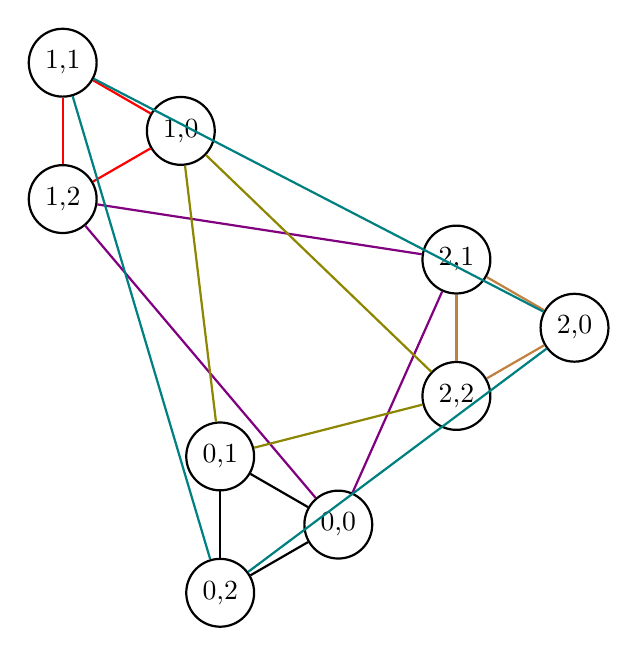
\begin{tikzpicture}
\begin{scope}[every node/.style={circle,thick,draw}]
\node (0) at (1,0)  {0,0}; 
\node (1) at (-.5, .866) {0,1}; 
\node (2) at  (-.5, -.866) {0,2}; 

\draw[thick, black] (0) -- (1); 
\draw[thick, black] (1) -- (2); 
\draw[thick, black] (0) -- (2); 

\node (3) at (-1,5)  {1,0}; 
\node (4) at (-2.5, 5.866) {1,1}; 
\node (5) at  (-2.5, 4.134) {1,2}; 

\draw[thick, red] (3) -- (4); 
\draw[thick, red] (4) -- (5); 
\draw[thick, red] (3) -- (5); 

\node (6) at (4,2.5)  {2,0}; 
\node (7) at (2.5, 3.366) {2,1}; 
\node (8) at  (2.5, 1.634) {2,2}; 

\draw[thick, brown] (6) -- (7); 
\draw[thick, brown] (7) -- (8); 
\draw[thick, brown] (6) -- (8); 

\draw[thick, violet] (0) -- (5); 
\draw[thick, violet] (5) -- (7); 
\draw[thick, violet] (0) -- (7); 


\draw[thick, olive] (1) -- (3); 
\draw[thick, olive] (3) -- (8); 
\draw[thick, olive] (1) -- (8); 


\draw[thick, teal] (2) -- (4); 
\draw[thick, teal] (4) -- (6); 
\draw[thick, teal] (2) -- (6); 


\end{scope}

\end{tikzpicture}
\label{fig:bipartite}
\caption{complete graphs with increment 2}
\end{figure}



\begin{figure}
\centering
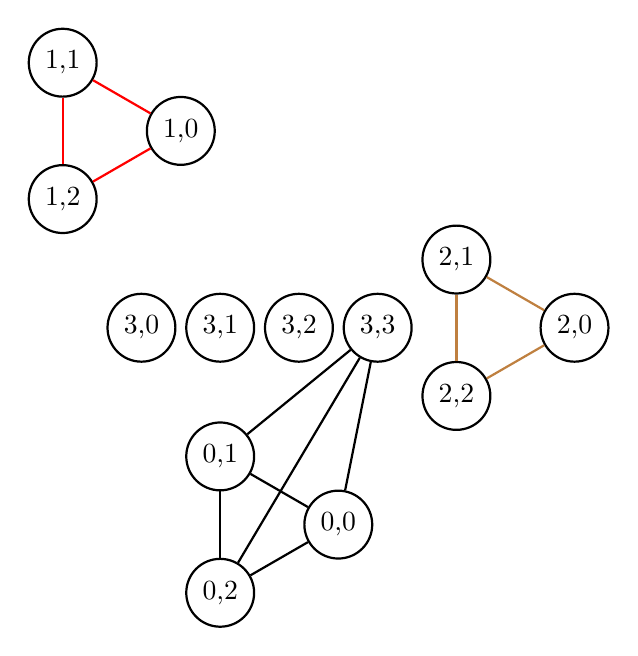
\begin{tikzpicture}
\begin{scope}[every node/.style={circle,thick,draw}]
\node (0) at (1,0)  {0,0}; 
\node (1) at (-.5, .866) {0,1}; 
\node (2) at  (-.5, -.866) {0,2}; 

\draw[thick, black] (0) -- (1); 
\draw[thick, black] (1) -- (2); 
\draw[thick, black] (0) -- (2); 

\node (3) at (-1,5)  {1,0}; 
\node (4) at (-2.5, 5.866) {1,1}; 
\node (5) at  (-2.5, 4.134) {1,2}; 

\draw[thick, red] (3) -- (4); 
\draw[thick, red] (4) -- (5); 
\draw[thick, red] (3) -- (5); 

\node (6) at (4,2.5)  {2,0}; 
\node (7) at (2.5, 3.366) {2,1}; 
\node (8) at  (2.5, 1.634) {2,2}; 

\draw[thick, brown] (6) -- (7); 
\draw[thick, brown] (7) -- (8); 
\draw[thick, brown] (6) -- (8); 


\node (9) at (-1.5, 2.5) {3,0};
\node (10) at (-.5, 2.5) {3,1};
\node (11) at (.5, 2.5) {3,2};
\node (12) at (1.50, 2.5) {3,3};

\draw[thick, black] (12) -- (0); 
\draw[thick, black] (12) -- (1); 
\draw[thick, black] (12) -- (2); 

\end{scope}
\end{tikzpicture}
\label{fig:bipartite}
\caption{$s=4, g=4, n=13, m=13$: adding to original cliques - 3,3 adds to each original}
\end{figure}

\begin{figure}
\centering
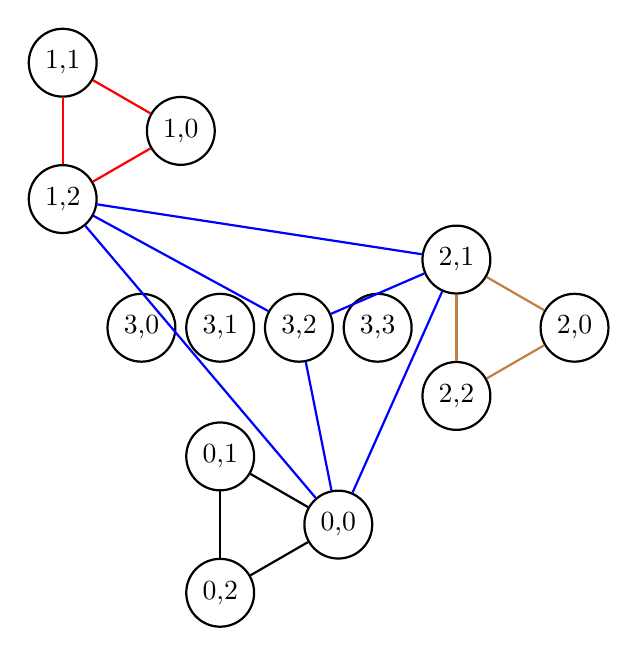
\begin{tikzpicture}
\begin{scope}[every node/.style={circle,thick,draw}]
\node (0) at (1,0)  {0,0}; 
\node (1) at (-.5, .866) {0,1}; 
\node (2) at  (-.5, -.866) {0,2}; 

\draw[thick, black] (0) -- (1); 
\draw[thick, black] (1) -- (2); 
\draw[thick, black] (0) -- (2); 

\node (3) at (-1,5)  {1,0}; 
\node (4) at (-2.5, 5.866) {1,1}; 
\node (5) at  (-2.5, 4.134) {1,2}; 

\draw[thick, red] (3) -- (4); 
\draw[thick, red] (4) -- (5); 
\draw[thick, red] (3) -- (5); 

\node (6) at (4,2.5)  {2,0}; 
\node (7) at (2.5, 3.366) {2,1}; 
\node (8) at  (2.5, 1.634) {2,2}; 

\draw[thick, brown] (6) -- (7); 
\draw[thick, brown] (7) -- (8); 
\draw[thick, brown] (6) -- (8); 


\node (9) at (-1.5, 2.5) {3,0};
\node (10) at (-.5, 2.5) {3,1};
\node (11) at (.5, 2.5) {3,2};
\node (12) at (1.50, 2.5) {3,3};

\draw[thick, blue] (0) -- (5); 
\draw[thick, blue] (5) -- (7); 
\draw[thick, blue] (0) -- (7); 


\draw[thick, blue] (11) -- (0); 
\draw[thick, blue] (11) -- (5); 
\draw[thick, blue] (11) -- (7); 


\end{scope}
\end{tikzpicture}
\label{fig:bipartite}
\caption{adding to increment cliques  - 3,2 adds to all 2 increment cliques}
\end{figure}






\begin{figure}
\centering
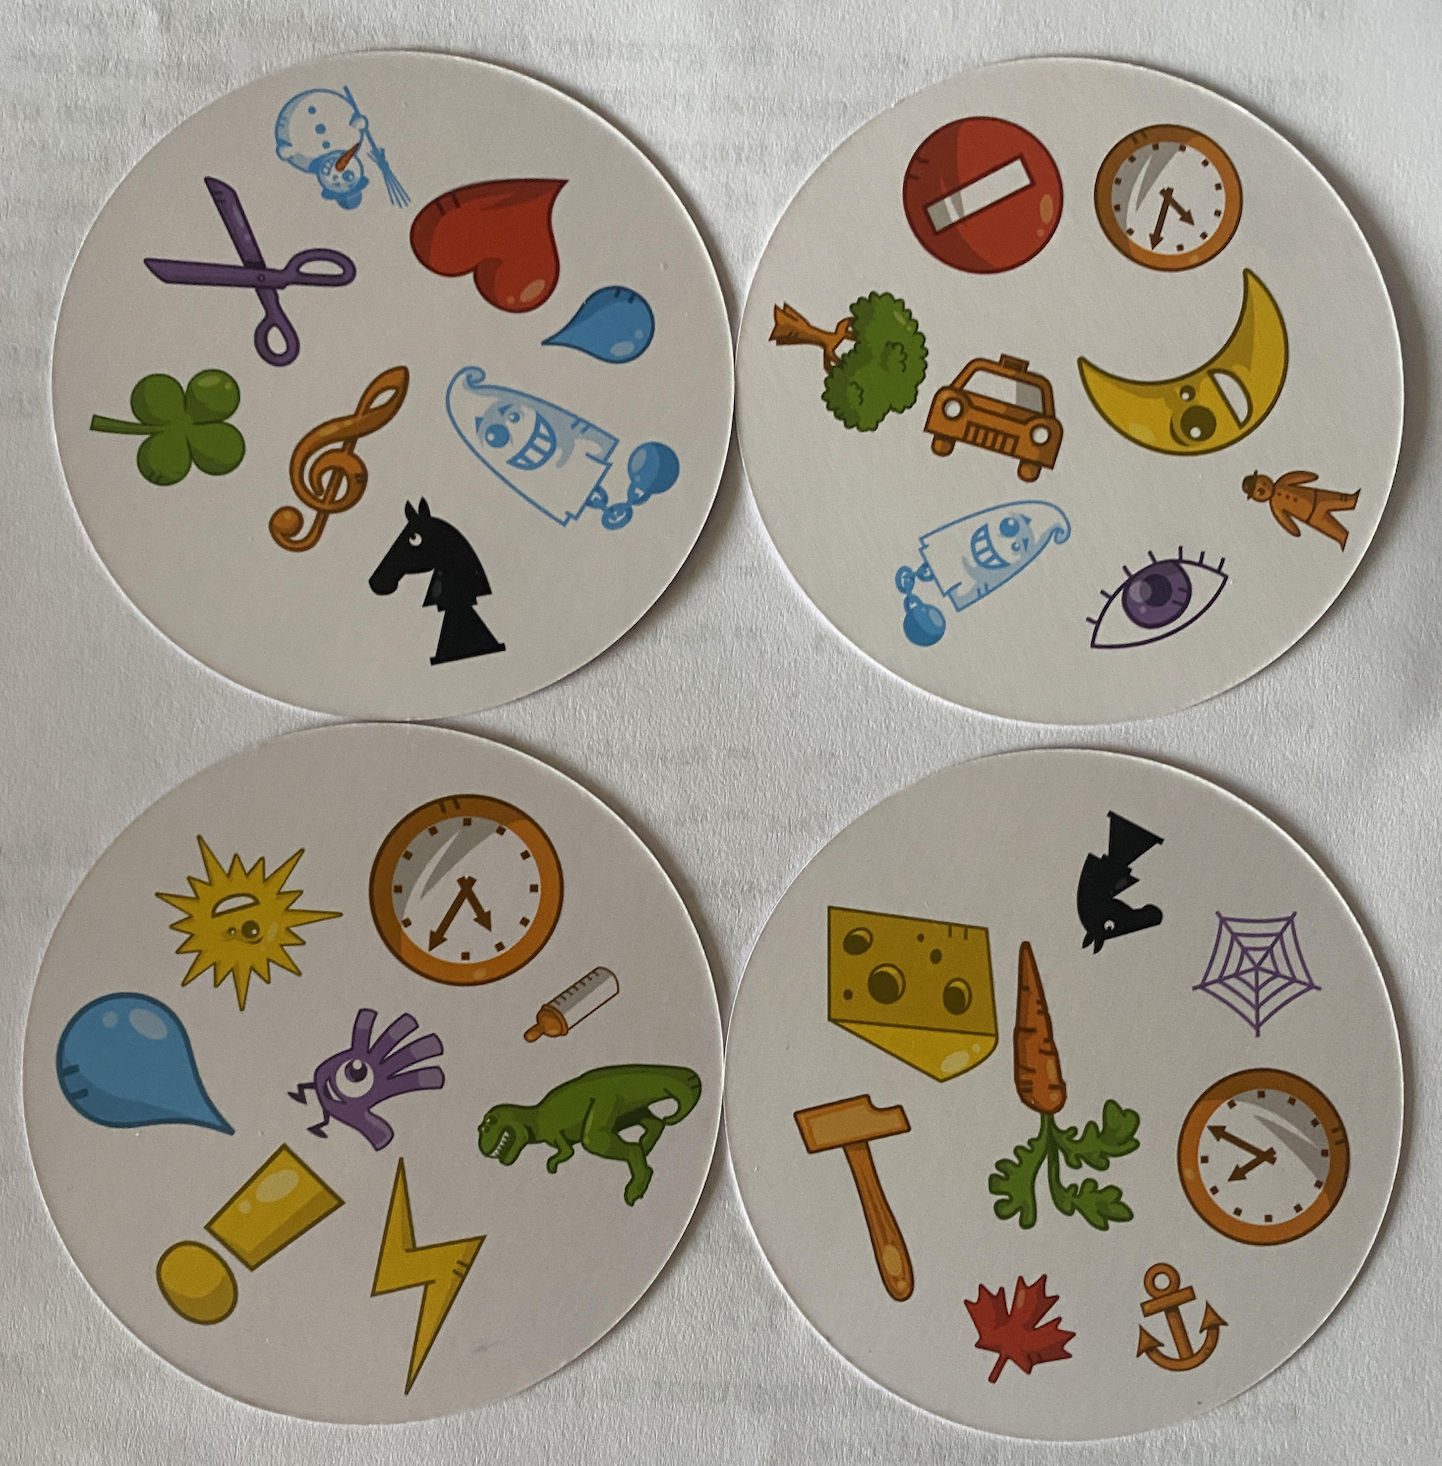
\includegraphics[scale=.3]{cards}
\caption{Dinosaur Cards}
\end{figure}

Children's games need to be simple. The game \emph{Memory} has seen innumerable rebranded recreations, because the mechanic is approachable (and nominally educational) and it can be sold repeatedly, with cartoon characters, animals, or whatever to engage a short attention span. A set of \emph{Memory} comes with matched pairs of cards with identical backs. Once the main mechanic is exhausted, the enterprising child will find some other game to create with this set. Here is that game, \emph{Dinosaur War}, created with the cards like those in Figure 1.

\subsection{Rules of Dinosaur War}

\begin{itemize} 
\item Players establish a ranking of cards, preferably under the direction of an opinionated child. Those might be ``Baryonyx beats Mosasaurus beats T-Rex... beats Apatosaurus'' in Figure 1, or the commonly-accepted Ace-to-2 if using a deck of playing cards.
\item Two players each get an identical deck of these cards. Cards were unique in this set but need not be. Players conceal their hand (though the content of the hands is well-known to those tracking it).
\item At each turn:
\begin{itemize}
\item Each player simultaneously plays a card face up.
\item The player whose card outranks the other's gets one point. If there is a tie, no points are awarded. The two played cards are set aside.
\item Play continues until the cards are exhausted.
\end{itemize}
\item The player with the most points at the end wins.
\end{itemize}

The maximum score individual score is 9 (since your opponent's 10 cannot be beaten, only tied). Game ties are relatively common. 

\subsection{``Strategy'' in Dinosaur War}

Intuitively, your hand has a certain amount of ``power'' that you deploy to beat an opponent; spending the minimum amount of ``power'' to win preserves better cards for later. 

Imagine on the first turn of a 10 card deck game with hands $A=B=\{1, 2, ... 10\}$, players $(P_A, P_B)$ play respective cards $(9, 10)$. This means:
\begin{itemize}
\item $P_B$ takes a one-point lead.
\item The 10 card is preserved for $P_A$. They will necessarily win one hand in the future.
\item The powerful 9 card is lost for $P_A$.
\end{itemize}

Alternatively, imagine the first move is $(1,10)$. This means:

\begin{itemize}
\item $P_B$ takes a one-point lead.
\item 10 is preserved for $P_A$. They will necessarily win one hand in the future.
\item 1 is lost for $P_A$, the worst card in the hand.
\item Each card of $P_A$'s hand beats at least one card in $P_B$'s hand.
\end{itemize}

The second scenario \emph{seems} better for $P_A$.\footnote{In this paper, we measure goodness by expected tricks taken by the hand.} But how much better? And how can one strategically strive to lose bad cards and win ``by just enough'' to take tricks? This is the focus of the paper.

\subsection{A reduced example}

Throughout, we'll use the following conventions:
\begin{itemize}
\item $P_A$'s available options are listed in bold down the left column of the payoff matrix (Fig 2a, 2b).
\item $P_B$'s available options are listed in bold across the top row.
\item A trick has a payoff of $1$ if $P_A$ wins, and $-1$ if $P_B$ wins. $P_A$ is trying to get the total score as high above zero as possible, $P_B$ below.
\item For a payoff matrix $M$, the cell at row $i$, column $j$ is the value of that trick, plus the expected value of the remaining game.
\end{itemize}


This is easy to see in Fig 2a, where the hands are identical. There are only four games of $(P_A, P_B)$ move pairs:
\begin{itemize}
\item $(1,1)$ means the first trick payoff is zero, and the rest of the game (necessarily $(3,3)$) is determined, also of payoff zero.
\item $(3,3)$ follows similarly.
\item $(3,1)$ means the first trick payoff is 1, and the rest of the game (necessarily $(1,3)$) pays off -1, for a total of zero.
\item $(1,3)$ follows in reverse, with another time game.
\end{itemize}

It's clear that \emph{any strategy} is equivalent in this very boring small game. $P_A$ could even announce his moves before $P_B$ selects a card, and the result of the game is still determined. The expected (and only possible )value of this game is zero.

Observe in figure 2b that starting sets $A =\{1,5\}, B= \{3,4\}$, while not identical, also yield this result; the choices don't matter in the end.

But for some uneven sets of cards, like in Fig 2c, things are different.
\begin{itemize}
\item If $P_A$ is able to play their 2 against a 1 (on either first or second trick), they win both tricks for a score of 2.
\item If $P_A$ plays their 2 against a 3, this trick score is -1, but guaranteed to balance by the imminent (or recently played) $(4,1)$ trick, for a total of 0.
\end{itemize}

This is more like \emph{Rock-Scissors-Paper}: knowing your opponent's choice wins you the game. And, like RSP, the mere existence of better choices does not mean that there exists a perfect-information strategy with a nonzero expected value.

How can we quantify the goodness of one hand versus another? We introduce a metric for this particular game called the \emph{Dominance Score}\footnote{This should not be conflated with a \emph{dominant} Nash strategy.}  and use this to compute the expected value of more complicated (larger) games.

\begin{figure}
\centering
\begin{subfigure}{.5\textwidth}
 \centering
$ \left[\begin{array}{ccc}
            & \mathbf{1} & \mathbf{3}\\ 
            \mathbf{1} & 0 & 0\\
            \mathbf{3} & 0 & 0\\
           \end{array}\right] 
$
 \caption{Even 2x2 game}
\label{fig:even_2x2}
\end{subfigure}

\begin{subfigure}{.5\textwidth}
 \centering
$ \left[\begin{array}{ccc}
            & \mathbf{3} & \mathbf{4}\\ 
            \mathbf{1} & 0 & 0\\
            \mathbf{5} & 0 & 0\\
           \end{array}\right] 
$
 \caption{Another even 2x2 game}
\label{fig:another_even_2x2}
\end{subfigure}

\begin{subfigure}{.5\textwidth}
 \centering
$ \left[\begin{array}{ccc}
            & \mathbf{1} & \mathbf{3}\\ 
            \mathbf{2} & 2 & 0\\
            \mathbf{4} & 0 & 2\\
           \end{array}\right] 
$
 \caption{Uneven 2x2 game}
\label{fig:uneven_2x2}
\end{subfigure}
\caption{Simple 2x2 games}
\label{fig:2x2}
\end{figure}


\section{Dominance Score}

The dominance score of two equal-sized sets (hands) $A = \{a_1, a_2, ... a_n\}, B = \{a_1, a_2, ... a_n\}$ is defined as \fbox{D(A,B) = $\sum_{i=1}^n \sum_{j=1}^n T(a_i, b_j)$}, where	

\[  
T(a,b) = 
   \begin{cases}
    1 & a > b\\
    0 & a = b \\
    -1 & a < b \\ 
   \end{cases}
\]

This is just adding up all possible winning tricks for $A$ and subtracting all possible winning tricks for $B$, ignoring ties. For example, if $A = \{2, 3,6\}, B = \{1,3,5\}$, then $D(A,B) = [T(2,1) + T(3,1) + T(6,1) + T(6,3) + T(6,5)] + [T(3,3)] +  [T(2,3) + T(2,5) + T(3,5)] = 5 + 0 - 3 = 2$.


\begin{itemize}
\item The identical hands in figure 2a necessarily have a dominance score of zero.
\item Figure 2b's pair of a hand with the 2nd- and 3rd-highest cards versus one with the lowest and highest rank, also has a dominance score of zero.
\item Figure 2c has a dominance score of two, so it's not surprising that the expected value of the game is in player A's favor (+2).
\end{itemize}


\begin{figure}
\centering
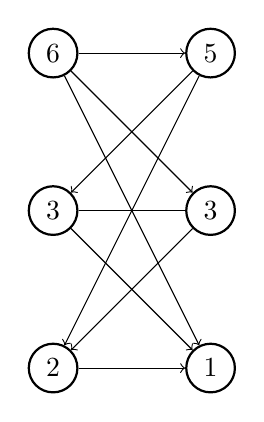
\begin{tikzpicture}
\begin{scope}[every node/.style={circle,thick,draw}]
  \node (1) at (0,0) {2};
  \node (2) at (0,2) {3};
  \node (3) at (0,4) {6};
  \node (4) at (2,0) {1};
  \node (5) at (2,2) {3};
  \node (6) at (2,4) {5};
\end{scope}

\draw[->] (1) -- (4); 
\draw[<-] (1) -- (5); 
\draw[<-] (1) -- (6); 
\draw[->] (2) -- (4); 
\draw[-] (2) -- (5); 
\draw[<-] (2) -- (6); 
\draw[->] (3) -- (4); 
\draw[->] (3) -- (5); 
\draw[->] (3) -- (6); 

\end{tikzpicture}
\label{fig:bipartite}
\caption{Dominance graph of $\{2,3,6\}$ vs. $\{1,3,5\}$}
\end{figure}

Another way to visualize hand $A$ against hand $B$ is a bipartite graph like Figure 3, counting ``right-pointing'' edges as +1, and ``left-pointing'' edges as -1. This shows that D($\{2,3,6\}$, $\{1,3,5\}) = 2$.



\section{Main Theorem and Proof Layout}

The main theorem we wish to prove states:

\begin{framed}
Given rational players, an optimal strategy in Dinosaur War is playing all options with uniform randomness.
\end{framed}

The steps to proving this are.

\begin{itemize}
\item Lemma 1: Across every row and column of the payoff matrix $M$ determined by hands $A$ and $B$, the entries sum to the graph's domination score $D(A,B)$.
\item Lemma 2: A payoff matrix of such a form of width $n$ has a Nash equilibrium\cite{2} of $p(a_i) = \frac{1}{n}, p(b_j) = \frac{1}{n}$ for all $i, j \in [1,n]$.
\item Lemma 3: The expected value of the game $A, B$ is then $\frac{D(A,B)}{n}$.
\end{itemize}

We will do this \emph{inductively} and \emph{simultaneously}, in that, if Lemma 1, 2, and 3 are true for boards of size $n-1$ and below, then we can prove them for a board of size $n$.

Additionally: There are no equilibria with a higher expected value in the game, since according to Von Neumann's Minimax theorem\cite{3}, all Nash equilibria of a zero-sum game have the same value. So though there may be other equally good strategies (duplicate cards in a hand allows the strategy to play \emph{one} versus the \emph{other} with some variation; also see the fait accompli games of Figure 2a, 2b), there are none more optimal than a uniform strategy.


Finally, we compute our payoff matrix for a larger game of card sets $A = B = [1,10]$.

\section{Lemmas: Base case}



\subsubsection{Base cases} 
\emph{Base case, n=1}: We see in Figure 4a that $D$ is equal to function $H$ at $n=1$: a 1 if player $A$'s single card outranks $B$'s, a 0 for a tie, and a $-1$ if $B$'s outranks. With a single element and therefore single row and column, the Lemma 1 is clearly true. There is only one total strategy in the game, so Lemma 2 is true. And Lemma 3 is equivalent to Lemma 1 when $n=1$.

\emph{(Extra) base case, n=2}: To see how this extends to a 2x2 matrix, consider Fig. 4b displaying the payoff matrix built from hands $A = (a_1, a_2) = \{3, 6\}; B = (b_1,b_2) = \{3,5\}$.

\begin{itemize}
\item The upper-left element is $T(a_1, b_1) + D(\{a_2\}, \{b_2\}) = T(a_1, b_1) + T(a_2, b_2)$
\item The upper-right element is $T(a_1, b_2) + D(\{a_2\}, \{b_1\}) = T(a_1, b_2) + T(a_2, b_1)$
\item The lower-left element is $T(a_2, b_1) + D(\{a_1\}, \{b_2\}) = T(a_2, b_1) + T(a_1, b_2)$
\item The lower-right element is $T(a_2, b_2) + D(\{a_1\}, \{b_1\}) = T(a_2, b_2) + T(a_1, b_1)$
\end{itemize}

It is clear that summing the top row, bottom row, left column, or right column yields $T(a_1, b_1) + T(a_1, b_2) + T(a_2, b_1) + T(a_2, b_2) = D(A,B)$. 

At the 2x2 size, it should be clear that:
\begin{itemize}
\item The upper left and lower right values are necessarily equal, as are the upper right and lower left. There are four possible game sequences (completely determined by the first move), and those starting with, say, $(3,3)$ in figure 5b need to end with $(6,5)$, equivalent to $[(6,5), (3,3)]$.
\item Because of this identity, the rows and columns all sum to the same value. (proving Lemma 1 at $n=2$)
\item An equilibrium strategy of this zero sum game is playing each option with probability $\frac{1}{2}$, as the players are essentially playing a game of Matching Pennies\cite{1} (showing Lemma 2).
\item Therefore, the expected payoff is the average of a(ny) row or column (showing Lemma 3).
\end{itemize}



\begin{figure}
\centering
\begin{subfigure}{.5\textwidth}
 \centering
 

$ \left[\begin{array}{cc}
            & \mathbf{5}\\ 
            \mathbf{6} & 1\\
           \end{array}\right] 
$

 \caption{1x1 base case}
\label{fig:basecase_1x1}
\end{subfigure}
\begin{subfigure}{.5\textwidth}
 \centering

$ \left[\begin{array}{ccc}
            & \mathbf{3} & \mathbf{5}\\ 
            \mathbf{3} & 1 & 0\\
            \mathbf{6} & 0 & 1\\
           \end{array}\right] 
$
 \caption{2x2 base case}
\label{fig:basecase_1x1}
\end{subfigure}
\caption{Base cases}
\label{fig:base}
\end{figure}


\section{Inductive case}



\begin{figure}
\centering
\begin{subfigure}{.5\textwidth}
 \centering
 
\[
\left[ 
\begin{array}{c@{}c@{}c@{}c}
& \mathbf{1} & \mathbf{3} & \mathbf{5} \\


\mathbf{2} & \left[\begin{array}{ccc}
            & \mathbf{3} & \mathbf{5}\\ 
            \mathbf{3} & 1 & 0\\
            \mathbf{6} & 0 & 1\\
           \end{array}\right] 
           & \left[\begin{array}{ccc}
            & \mathbf{1} & \mathbf{5}\\ 
            \mathbf{3} & 2 & 0 \\
            \mathbf{6} & 0 & 2 \\
           \end{array}\right]  
           & \left[\begin{array}{ccc}
            & \mathbf{1} & \mathbf{3}\\ 
            \mathbf{3} & 2 & 1 \\
            \mathbf{6} & 1 & 2 \\
           \end{array}\right]  \\           
           
 \mathbf{3} & \left[\begin{array}{ccc}
            & \mathbf{3} & \mathbf{5}\\ 
            \mathbf{2} &0 & 0 \\
            \mathbf{6} & 0 & 0 \\
           \end{array}\right]
           & \left[\begin{array}{ccc}
            & \mathbf{1} & \mathbf{5}\\ 
            \mathbf{2} & 2 & 0 \\
            \mathbf{6} & 0 & 2 \\
           \end{array}\right]  
           & \left[\begin{array}{ccc}
            & \mathbf{1} & \mathbf{3}\\ 
            \mathbf{2} & 2 & 0 \\
            \mathbf{6} & 0 & 2 \\
           \end{array}\right]  \\             
           
           
\mathbf{6} & \left[\begin{array}{ccc}
            & \mathbf{3} & \mathbf{5}\\ 
            \mathbf{2} & -2 & -1 \\
            \mathbf{3} & -1 & -2 \\
           \end{array}\right] 
& \left[\begin{array}{ccc}
            & \mathbf{1} & \mathbf{5}\\ 
            \mathbf{2} & 0 & 0 \\
            \mathbf{3} & 0 & 0 \\
           \end{array}\right]  
           & \left[\begin{array}{ccc}
            & \mathbf{1} & \mathbf{3}\\ 
            \mathbf{2} & 1 & 0 \\
            \mathbf{3} & 0 & 1 \\
           \end{array}\right]  \\  
\end{array}\right]
\]  
 \caption{Recursive game matrix}
\label{fig:236135_recursive}
\end{subfigure}

\begin{subfigure}{.5\textwidth}
\[
\left[ 
\begin{array}{c@{}c@{}c@{}c}
& \mathbf{1} & \mathbf{3} & \mathbf{5} \\


\mathbf{2} & (\mathit{1} + .5 = 1.5) & (\mathit{-1} + 1 = 0) & (\mathit{-1} + 1.5 = .5) \\
\mathbf{3} & (\mathit{1} +0 = 1) & (\mathit{0} + 1 = 1) & (\mathit{-1} + 1 = 0) \\             
 \mathbf{6} & (\mathit{1} + -1.5 = -.5) & (\mathit{1} + 0 = 1) & (\mathit{1} + .5 = 1.5) \\
\end{array}\right]
\]  
\caption{Payoff matrix}
\label{fig:236135_payoff}
\end{subfigure}

\caption{$\{2,3,6\}$ vs. $\{1,3,5\}$}
\label{fig:236135}
\end{figure}



For the \emph{inductive case}, consider Figure 5a and Figure 5b. In each, the vertical axis is the set of moves $A$ for player $P_A$, and the horizontal the move set $B$ for player $P_B$.

In Figure 5a, the element $(i,j)$ represents the game continuation (or subgame) should the next play be $(a_i, b_j)$ (so, excluding cards $a_i$ and $b_j$). 
In Figure 5b, the element $(i,j)$ is of the form (``immediate payoff from move $(a_i, b_j)$'' and ``expected payoff of remaining subgame''). So, the upper right element of 5b is $(\mathit{1} + .5 = 1.5)$; the italicized 1 represents that card 2 beats card 1. .5 points is the expected payoff of the subgame $\{3,6\}$ vs. $\{3,5\}$, totaling 1.5. 

\subsection{Inductive case for Lemma 1}

In 5a, the subgame at $(i, j)$ is the full game $(A - \{a_i\}, B-\{b_j\})$. This is ``the rest of the game'' with cards $a_i, b_j$ already used up. By inductive hypothesis, the payoff of the game at matrix entry $(1,1)$ is $D(A-\{a_i\}, B-\{b_j\})$, which is the sum of $T(a_m, b_n)$ for all combinations of $m, n$ except all those where $m=i$ or $n=j$. 

Without loss of generality, consider row $a_1$ ($P_A$ plays card 2) in Figure 5a (the subgames) and in figure 5b. Note that for $i=1$, summing across all expected subgame payoffs $\frac{D(A-\{a_1\}, B-\{b_j\})}{n-1}$ counts each pair $T(a_i, b_j), i \neq 1$ exactly $n-1$ times. $a_i, i \neq 1$ is always in each subgame, and $b_j$ is in every subgame except those in column $j$, for a total of $n-1$. So, with each $D$ term fully expanded, the sum includes $n-1$ terms $\frac{T(a_i, b_j)}{n-1}, i \neq 1$. These correspond to the numbers on the right side of the addition sign in figure 5b.

The immediate payoffs of playing $a_1$ (card 2 in this case) are just $T(a_1, b_1), T(a_1, b_2)... T(a_1, b_n)$, corresponding to the (italicized) number on the left side of the addition sign in 5b. Of course, summing the immediate payoffs ($\sum_{i=2}^n\sum_{j=1}^n T(a_i, b_j)$) and the subgame payoffs ($\sum_{j=1}^n T(a_1 b_j)$) is the definition of $D(A,B)$. This proves Lemma 1.

This logic holds equivalently for any other row or any column.

\subsection{Lemma 2}

Consider a payoff matrix where each row and each column sum to the same value (in our case, this is always $D(A,B)$).

A Nash equilibrium occurs for players $P_A, P_B$ when any deviation of $P_A$ from the equilibrium benefits $P_B$, assuming $P_A$ announces his strategy (and same for $P_B, P_A$).

Assume both strategies are uniform: $p(a_1) = p(a_2) = .... = \frac{1}{n} = p(b_1) = p(b_2) = ... p(b_n)$. Then the payoff of any given row $i$ would be, by Lemma 1, $\sum_{j=1}^n M_{i,j} = n \cdot \frac{1}{n} D(A,B) = D(A,B)$; the same follows for columns. The sum of all payoffs across the matrix is then $n \cdot D(A,B)$.

If $P_A$ shifts his strategy to a different distribution $p(a_1), p(a_2), ..., p(a_n)$, note that the sum of all payoffs $n\cdot D(A,B)$ does not change, since this is simply reallocating the probabilities, which sum to 1, over different rows each of expected value $D(A,B)$. 

\begin{itemize}
\item Case 1: If this reallocation sees each column $j$'s expected payoff $\sum_{i=1}^n M_{i,j} p(a_i)$  still summing to $D(A,B)$, then the equilibrium condition (and the same expected payoff) is maintained. 
\item Case 2: If, however, a column $j$ sums to a value greater than $D(A,B)$, then $p(b_j) = 1; p(b_k) = 0$ for $(k \neq j)$ increases $P_B$'s payoff. As a zero-sum game, this decreases $P_A$'s payoff, and $P_A$ would not choose it. Note that if Case 1 does not hold, there \emph{must} be a column like $j$, since the sum across all columns remains $n \cdot D(A,B)$. In other words, if we're not in Case 1, column sums can't all be less than or equal to $D(A,B)$, or the sum wouldn't be $n \cdot D(A,B)$, so at least one column has a payoff greater than $D(A,B)$.
\end{itemize}


With Lemma 2 proven, Lemma 3 follows quickly. Each $M_{i,j}$ occurs with probablity $\frac{1}{n^2}$, and the matrix entries sum to $n \cdot D(A,B)$, so the expected payoff is $\frac{D(A,B)}{n}$.




\section{Considerations and Examples}

Computing the expected value of the matrices in Figure 5a recursively gets computationally expensive, but with this formula in hand, the code \footnote{\url{https://github.com/fettermania/mathnotes/tree/main/dino/clj/dino/src/dino/core.clj}} becomes very simple: just apply Lemmas 1-3, and the 10 v. 10 game payoffs are easily generated (Figure 6).

Note that:

\begin{itemize}
\item The matrix is obviously symmetric.
\item Winning the first trick is neither a net positive nor negative.
\item Winning by exactly ($n/2$) rank spots is neutral; winning a trick by less than that yields a net positive value (for player $P_A$), and more than that, a negative value.
\end{itemize}
\begin{figure}
\centering
\setcounter{MaxMatrixCols}{20}

$\begin{bmatrix}
& \mathbf{1} & \mathbf{2} & \mathbf{3} & \mathbf{4} & \mathbf{5} & \mathbf{6} &\mathbf{7} & \mathbf{8} &\mathbf{9} & \mathbf{10} \\ 
\mathbf{1} & 0 & -8/9 & -2/3 & -4/9 & -2/9 & 0 & 2/9 & 4/9 & 2/3 & 8/9 \\
\mathbf{2} & 8/9 & 0 & -8/9 & -2/3 & -4/9 & -2/9 & 0 & 2/9 & 4/9 & 2/3 \\
\mathbf{3} & 2/3 & 8/9 & 0 & -8/9 & -2/3 & -4/9 & -2/9 & 0 & 2/9 & 4/9 \\
\mathbf{4} & 4/9 & 2/3 & 8/9 & 0 & -8/9 & -2/3 & -4/9 & -2/9 & 0 & 2/9 \\
\mathbf{5} & 2/9 & 4/9 & 2/3 & 8/9 & 0 & -8/9 & -2/3 & -4/9 & -2/9 & 0 \\
\mathbf{6} & 0 & 2/9 & 4/9 & 2/3 & 8/9 & 0 & -8/9 & -2/3 & -4/9 & -2/9 \\
\mathbf{7} & -2/9 & 0 & 2/9 & 4/9 & 2/3 & 8/9 & 0 & -8/9 & -2/3 & -4/9 \\
\mathbf{8} & -4/9 & -2/9 & 0 & 2/9 & 4/9 & 2/3 & 8/9 & 0 & -8/9 & -2/3 \\
\mathbf{9} & -2/3 & -4/9 & -2/9 & 0 & 2/9 & 4/9 & 2/3 & 8/9 & 0 & -8/9 \\
\mathbf{10} & -8/9 & -2/3 & -4/9 & -2/9 & 0 & 2/9 & 4/9 & 2/3 & 8/9 & 0 \\
\end{bmatrix}
$

\caption{$A = B = [1,10]$ payoff matrix}
\label{fig:236135}
\end{figure}


Though the double-uniform strategy is optimal, and no other perfect information strategies outperform it (Lemma 2), certainly, like \emph{Rock-Scissors-Paper}, having an inkling of what the opponent will do can yield advantage. 

Note again that there are cases where the choice of move truly does not matter, (like fig 2a and 2c), or, in some version of the game, where $k$ duplicate cards could render the choice between them irrelevant (as long as the sum of the probabilities remains $\frac{k}{n}$.

This paper has only dealt with the expected value of the game, not the chance of winning, though my intuition is that this would follow similarly\footnote{Though this is not a proof!}.



% \begin{thebibliography}{9}
% \bibitem{1} Wikipedia: \url{https://en.wikipedia.org/wiki/Matching_pennies}
%\bibitem{2} Wikipedia: \url{https://en.wikipedia.org/wiki/Nash_equilibrium}
%\bibitem{3} Wikipedia: \url{https://en.wikipedia.org/wiki/Minimax_theorem}
%\end{thebibliography}

\end{comment}

\begin{thebibliography}{9}
\bibitem{1} Wikipedia: \url{https://en.wikipedia.org/wiki/Brooks\%27_theorem}
\end{thebibliography}

\end{document}

% == Boneyard: Extra exmaple of a payoff matrix in 3x3. ==
\begin{comment}

\begin{figure}
\centering
\begin{subfigure}{.5\textwidth}
 \centering
 
\[
\left[ 
\begin{array}{c@{}c@{}c@{}c}
& \mathbf{1} & \mathbf{3} & \mathbf{6} \\
\mathbf{2} & \left[\begin{array}{ccc}
            & \mathbf{3} & \mathbf{6}\\ 
            \mathbf{3} & 0 & 0\\
            \mathbf{6} & 0 & 0\\
           \end{array}\right] 
           & \left[\begin{array}{ccc}
            & \mathbf{1} & \mathbf{6}\\ 
            \mathbf{3} & 1 & 0 \\
            \mathbf{6} & 0 & 1 \\
           \end{array}\right]  
           & \left[\begin{array}{ccc}
            & \mathbf{1} & \mathbf{3}\\ 
            \mathbf{3} & 2 & 1 \\
            \mathbf{6} & 1 & 2 \\
           \end{array}\right]  \\           
           
 \mathbf{3} & \left[\begin{array}{ccc}
            & \mathbf{3} & \mathbf{6}\\ 
            \mathbf{2} &-1 & 0 \\
            \mathbf{6} & 0 & -1 \\
           \end{array}\right]
           & \left[\begin{array}{ccc}
            & \mathbf{1} & \mathbf{6}\\ 
            \mathbf{2} & 1 & 0 \\
            \mathbf{6} & 0 & 1 \\
           \end{array}\right]  
           & \left[\begin{array}{ccc}
            & \mathbf{1} & \mathbf{3}\\ 
            \mathbf{2} & 2 & 0 \\
            \mathbf{6} & 0 & 2 \\
           \end{array}\right]  \\             
           
           
\mathbf{6} & \left[\begin{array}{ccc}
            & \mathbf{3} & \mathbf{6}\\ 
            \mathbf{2} & -2 & -1 \\
            \mathbf{3} & -1 & -2 \\
           \end{array}\right] 
& \left[\begin{array}{ccc}
            & \mathbf{1} & \mathbf{6}\\ 
            \mathbf{2} & 0 & 0 \\
            \mathbf{3} & 0 & 0 \\
           \end{array}\right]  
           & \left[\begin{array}{ccc}
            & \mathbf{1} & \mathbf{3}\\ 
            \mathbf{2} & 1 & 0 \\
            \mathbf{3} & 0 & 1 \\
           \end{array}\right]  \\  
\end{array}\right]
\]  
 \caption{Recursive game matrix}
\label{fig:236136_recursive}
\end{subfigure}

\begin{subfigure}{.5\textwidth}
\[
\left[ 
\begin{array}{c@{}c@{}c@{}c}
& \mathbf{1} & \mathbf{3} & \mathbf{6} \\


\mathbf{2} & (\mathit{1} + 0 = 1) & (\mathit{-1} + .5 = -.5) & (\mathit{-1} + 1.5 = .5) \\
\mathbf{3} & (\mathit{1} -.5 = .5) & (\mathit{0} + .5 = .5) & (\mathit{-1} + 1 = 0) \\             
 \mathbf{6} & (\mathit{1} -1.5 = -.5) & (\mathit{1} + 0 = 1) & (\mathit{0} + .5 = .5) \\
\end{array}\right]
\]  
\caption{Payoff matrix}
\label{fig:236136_payoff}
\end{subfigure}

\caption{$\{2,3,6\}$ vs. $\{1,3,6\}$}
\label{fig:236136}
\end{figure}
\end{comment}$s \equiv 0 mod 3$, 

